\begin{frame}{Proposta}
    % \begin{itemize}
    %     \item \citeonline{rigon2020inferring} estabelecem o núcleo de uma linguagem funcional pura com sintaxe imperativa em que é possível declarar novos tipos de dados para representar efeitos.

    %     \item []

    %     \item [] \begin{figure}
    %         \centering
    %         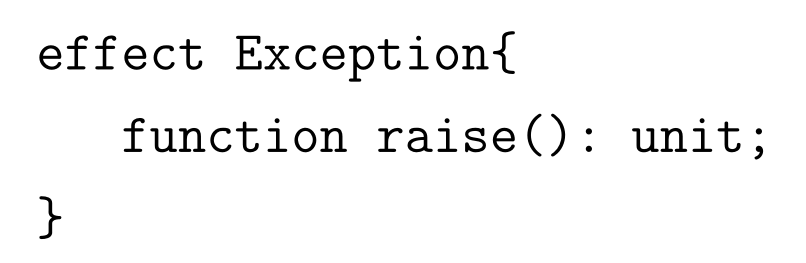
\includegraphics[width=.6\textwidth]{Figuras/excep.png}
    %         \caption{Declaração do efeito \textit{Exception}}
    %         \label{fig:exc}
    %     \end{figure}

    %     \item Possível tradução: Mônada \textit{Maybe}

    % \end{itemize}
\end{frame}

\begin{frame}{Conclusões Parciais}
    % \begin{itemize}
    %     \item Fundamentação teórica
    %     \item Como uma possível alternativa a tradução apresentada por \citeonline{vazou2016monads}, para tratar \textit{row-effects} de forma mais elegante, será investigada a viabilidade de utilizar mônadas livres \cite{kiselyov2015freer}
    % \end{itemize}
\end{frame}